\chapteropen{Chapter 7: Software process models}{chapter-7}
\markboth{Ch. 7 | Processes}{}


\begin{studycolumns}
\vspace{0pt}
\begin{eli5box}
Waterfall is like planning a whole house before construction; incremental delivery is like opening usable rooms in stages; reuse/\allowbreak{}configuration is like assembling suitable existing modules. None is automatically best. Choose according to change, risk, available components and the need for predictable agreement.
\end{eli5box}
\textbf{Answer check:} Choose using change, risk, component fit and constraints. Give a case-specific benefit and trade-off. Waterfall includes testing; agile includes planning. Customer involvement does not eliminate the cost of late change.
\end{studycolumns}

\subsection*{Visual: compare how the work is arranged}
\sectionlabel{h-visual-compare-how-the-work-is-arranged}


\par\smallskip\noindent\begin{minipage}{\linewidth}\centering
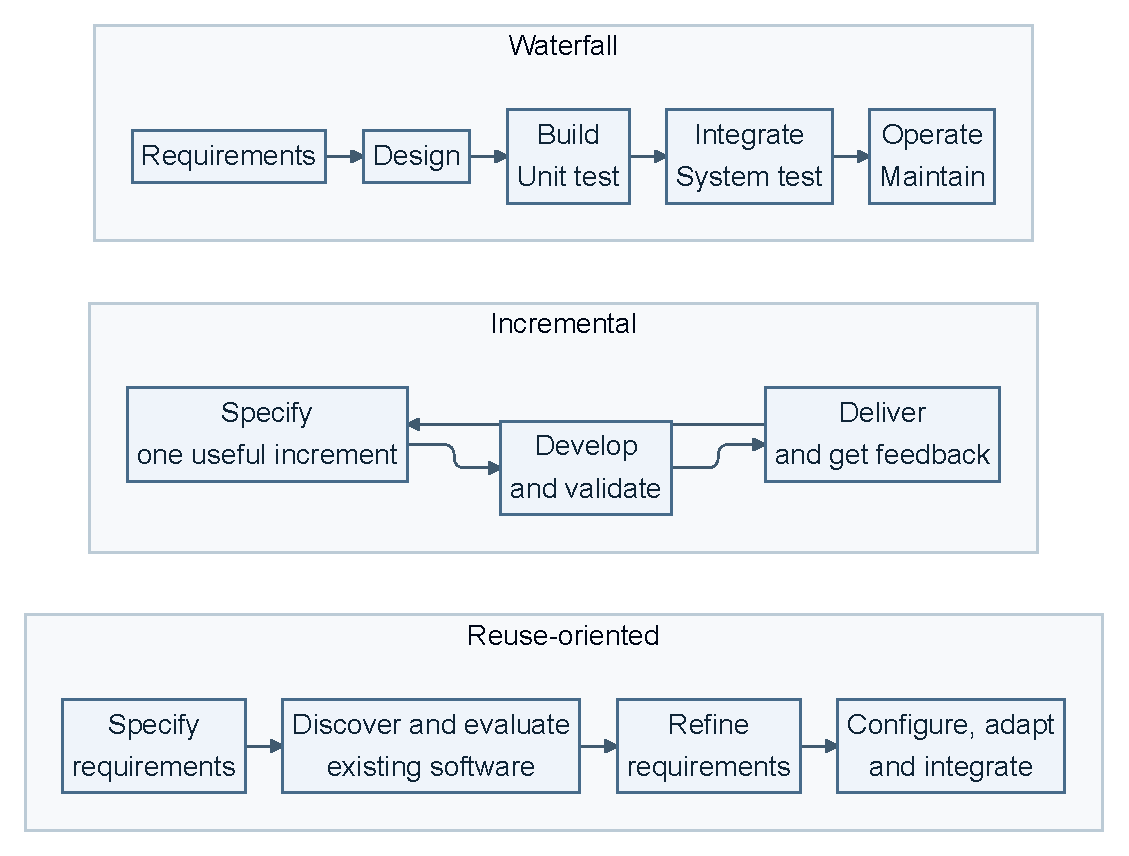
\includegraphics[width=332.12pt]{images/fig-022.pdf}
\captionof{figure}{compare how the work is arranged}\end{minipage}\par\smallskip

\begin{studycolumns}
\vspace{0pt}



\needspace{4\baselineskip}
\subsection*{7.1 Definitions}
\sectionlabel{h-71-definitions}

\begin{quote}\small\color{navy}
A \textbf{software process} is \emph{a structured set of activities required to develop a software system.}

\end{quote}
All processes involve specification, design/\allowbreak{}implementation, validation and evolution (Chapter 1). Their arrangement and feedback differ.

\begin{quote}\small\color{navy}
A \textbf{software process model} is \emph{an abstract representation of a process --- a description from some particular perspective.}

\end{quote}
\textbf{Process descriptions} include, besides activities and their ordering:

\begin{itemize}
\item \textbf{Products} --- outcomes of a process activity;
\item \textbf{Roles} --- responsibilities of the people involved;
\item \textbf{Pre- and post-conditions} --- statements true before/\allowbreak{}after an activity or product.
\end{itemize}
\end{studycolumns}

\Needspace{4\baselineskip}
\subsection*{7.2 Plan-driven vs agile}
\sectionlabel{h-72-plan-driven-vs-agile}


{\fontsize{9}{11}\selectfont
\begin{longtable}{L{\dimexpr 0.19914\linewidth-4.78pt\relax}L{\dimexpr 0.34730\linewidth-8.34pt\relax}L{\dimexpr 0.45356\linewidth-10.89pt\relax}}
\toprule
\rowcolor{ice}\textbf{} & \textbf{\textbf{Plan-driven}} & \textbf{\textbf{Agile}} \\
\midrule\endfirsthead
\toprule\rowcolor{ice}\textbf{} & \textbf{\textbf{Plan-driven}} & \textbf{\textbf{Agile}} \\
\midrule\endhead
\multicolumn{3}{r}{\scriptsize Continued on next page}\\\endfoot
\bottomrule\endlastfoot
Planning & All activities planned \textbf{in advance}; progress measured against the plan & Planning is \textbf{incremental}; process easily changed to reflect changing requirements \\
Iteration & Iteration occurs \textbf{within} activities & Specification, design, implementation, testing are \textbf{inter-leaved}; outputs negotiated during development \\
Outputs & Decided \textbf{up front} & Decided through \textbf{negotiation} during the process \\
\end{longtable}
}

Most practical processes include \textbf{elements of both}. \textbf{There are no right or wrong software processes.}


\Needspace{4\baselineskip}
\subsection*{7.3 The three general models}
\sectionlabel{h-73-the-three-general-models}


{\fontsize{9}{11}\selectfont
\begin{longtable}{L{\dimexpr 0.13392\linewidth-5.36pt\relax}L{\dimexpr 0.19287\linewidth-7.71pt\relax}L{\dimexpr 0.22020\linewidth-8.81pt\relax}L{\dimexpr 0.19571\linewidth-7.83pt\relax}L{\dimexpr 0.25730\linewidth-10.29pt\relax}}
\toprule
\rowcolor{ice}\textbf{Model} & \textbf{Shape} & \textbf{When used} & \textbf{Key benefit} & \textbf{Key problem} \\
\midrule\endfirsthead
\toprule\rowcolor{ice}\textbf{Model} & \textbf{Shape} & \textbf{When used} & \textbf{Key benefit} & \textbf{Key problem} \\
\midrule\endhead
\multicolumn{5}{r}{\scriptsize Continued on next page}\\\endfoot
\bottomrule\endlastfoot
\textbf{Waterfall} & Separate, distinct, sequential phases & Requirements \textbf{well understood} and changes limited; large systems-engineering projects developed at several sites & Plan-driven coordination across sites & \textbf{Difficulty of accommodating change} once under way; inflexible partitioning \\
\textbf{Incremental} & Specification, development, validation \textbf{inter-leaved}; may be plan-driven \textbf{or} agile & Most business systems & Lower cost of accommodating change; easier customer feedback; earlier delivery of value & \textbf{Process not visible} (managers need deliverables); \textbf{structure degrades} as increments are added unless you refactor \\
\textbf{Integration \& configuration (reuse-oriented)} & Assemble from existing components/\allowbreak{}COTS & Systems buildable from existing assets; standard for many business systems & Reduced cost and risk; faster delivery & \textbf{Requirements compromises inevitable}; loss of control over evolution of reused elements \\
\end{longtable}
}

\begin{studycolumns}
\vspace{0pt}

\textbf{Waterfall phases} (exact names): Requirements analysis and definition \ensuremath{\rightarrow} System and software design \ensuremath{\rightarrow} Implementation and unit testing \ensuremath{\rightarrow} Integration and system testing \ensuremath{\rightarrow} Operation and maintenance.


\textbf{Visibility note:} managers need regular deliverables, but documenting every version can be costly; refactoring controls the structural degradation identified in the table.

\textbf{Reuse-oriented phases (5):} requirements specification \ensuremath{\rightarrow} software discovery and evaluation \ensuremath{\rightarrow} requirements refinement \ensuremath{\rightarrow} application system configuration \ensuremath{\rightarrow} component adaptation and integration.

\textbf{Types of reusable software (3):} stand-alone application systems (COTS) configured for a particular environment; collections of objects packaged for a component framework (.NET, J2EE); web services developed to service standards and remotely invocable.


\begin{quote}\small\color{navy}
\textbf{Trap \#1.} "Incremental = agile" is \textbf{false} --- incremental development \emph{may be plan-driven}.


\end{quote}
\needspace{4\baselineskip}
\subsection*{7.4 Why costs are high /\allowbreak{} why maintenance dominates (Tutorial 4)}
\sectionlabel{h-74-why-costs-are-high--why-maintenance-dominates-tutorial-4}
Prepare a \emph{reasoned} answer, not a slogan:

\begin{itemize}
\item \textbf{Costs}: requirements churn, integration of heterogeneous components, testing effort grows super-linearly with interfaces, coordination cost in teams, environment/\allowbreak{}tooling/\allowbreak{}long lifetimes.
\item \textbf{Maintenance}: software is soft --- it \emph{can} change, so it \emph{must} change (new requirements, new platforms, bug fixes). Systems can live for decades; ongoing fixes and adaptation accumulate over that lifetime. Unlike hardware, there is no manufacturing cost, so evolution dominates total cost.
\item \textbf{Characteristics affecting development}: size (source/\allowbreak{}binary/\allowbreak{}users/\allowbreak{}developers/\allowbreak{}lifetime/\allowbreak{}versions), complexity (environment, technologies, hardware), cost and schedule constraints, non-functional requirements (performance, availability, security, scalability, extensibility).
\item \textbf{Two distinct differences from hardware manufacturing}: (1) software is \textbf{designed, not manufactured} --- copying is free; (2) software \textbf{does not wear out} --- it degrades by change, and hardware failures follow a bathtub curve.
\end{itemize}


\par\needspace{65pt}\phantomsection\label{answer-waterfall}
\textbf{Template W --- change/\allowbreak{}process answer:} clarify and record change; assess effects on requirements, design, code, tests, cost and schedule; agree revised scope/\allowbreak{}baselines; replan and verify. Early prototypes/\allowbreak{}reviews and increments expose change sooner, but do not remove late rework. Incremental delivery can be plan-driven or agile. For reuse, evaluate fixed-component fit, prototype risky integrations, negotiate acceptable compromises and isolate mismatches behind adapters.
\textbf{Comparison:} Waterfall favours stable baselines, sequential delivery and requirements/\allowbreak{}review/\allowbreak{}acceptance involvement; Agile favours reprioritised usable increments, frequent customer feedback and earlier adaptation.
\end{studycolumns}
